\documentclass[a4paper]{ctexbook}
\usepackage[margin=1in]{geometry}
\usepackage{amsmath}
\usepackage{amsthm} % proof
\usepackage{amssymb} % \mathbb
% \usepackage{amstext} % \text
\newtheorem{theorem}{定理}[chapter] %定理按章编号
\newtheorem{lemma}{引理}[chapter]
\newtheorem{property}{性质}[chapter]
\newtheorem{example}{例}[chapter]
\usepackage{listings}
\lstset{language=C++, basicstyle=\ttfamily, frame=lines}
\newcommand{\idx}{\mathrm{idx}}
\newcommand{\cost}{\mathrm{cost}}
\usepackage{subcaption}
\newcommand{\mpc}{\mathrm{MinPC}}
\usepackage{clrscode3e}
\newcommand{\match}{\mathrm{match}}
\newcommand{\slack}{\mathrm{slack}}
\begin{document}
  \chapter{图论高级算法}
  \section{最大流}
  最大流算法分成两大类:增广路(augmengting path)算法与预流推进(preflow-push)算法。
  这一节介绍的三个算法,都属于增广路算法。
  下面给出几个术语和定义。
  \subsubsection*{流网络}\label{notations}
  最大流问题(maximum flow problem)是网络流问题(network flow problem)的一种。网络流问题的研究对象是流网络(flow network),在某些文献中流网络也称作网络流图(network flow graph)。流网络$G=(V,E,c,s,t)$是一个有向图,$V$、$E$是其点集与边集,点和边的数目分别记作$n$、$m$。$c\colon V\times V\to \mathbb{N}$是边的容量函数,每条边$(u,v)\in E$都有一容量$c(u,v)\in \mathbb{N}$,若$(u,v)\notin E$则$c(u,v) = 0$。$s$和$t$是流网络中的两个特殊点,分别称作源点和汇点。为简便计,流网络简称「网络」或「图」,简记作$G=(V,E)$。

  自环在网络中无意义,我们规定图$G$中不含自环。%允许网络中有重边。
  下文在论述、证明关于网络流的原理、性质或定理时,为了表示上的方便,我们对流网络做出两条限定:
  \begin{enumerate}
    \item 图中不存在重边;\label{Restrict:1}
    \item 图中不存在反向边,即若$(u,v)\in E$,则$(v,u)\notin E$。\label{Restrict:2}
  \end{enumerate}
  这两条限定都不妨碍一般性。我们可以通过将容量相加把重边合为一条边,反向边可以通过新增一个节点来消除。请读者注意,上文所谓「表示上的方便」是指一条边可以通过两个端点唯一确定。下文我们要介绍的算法和代码可以处理含有重边或反向边的图,这两条限定都不是根本性的,仅仅是为了方便表述而已。

  \subsubsection*{流}
  流是满足下述两个性质的实值函数$f\colon V\times V\to\mathbb{R}$:
  \begin{description}
    \item[容量限制:]对任意$u,v \in V$,有 $0\le f(u,v)\le c(u,v)$。
    \item[流守恒:]对任意$u\in V-\{s,t\}$,有$\sum\limits_{v\in V}f(v,u)= \sum\limits_{v\in V}f(u,v)$
  \end{description}
  $f(u,v)$即边$(u,v)$上的流量,若$(u,v)\notin E$,$f(u,v) = 0$。
  从源点$s$到汇点$t$的总流量称作流$f$的值,记作$|f|$,不难得出
  $$|f| = \sum_{v\in V}f(s,v) - \sum_{v\in V}f(v,s)\text{,}$$
  最大流问题即在给定的网络$G$中求一个值最大的流。

  \subsection{增广路方法}\label{augmenting-path-method}
  增广路方法是求解最大流问题的一种方法。本章要介绍的三个最大流算法都是基于增广路方法的。增广路算法涉及三个重要概念:残量网络,增广路,割。
  \subsubsection*{残量网络}
  给定流网络$G=(V,E,c,s,t)$和$G$上的一个流$f$。残量网络$G_f=(V,E_f,c_f, s, t)$是由$G$和$f$所导出的一个网络,简记作$G_f=(V,E_f)$。首先定义残余容量$c_f$:
  \[
  c_f(u,v) =
  \begin{cases}
    c(u,v) - f(u,v) & \text{若$(u,v)\in E$,}\\
    f(v,u) & \text{若$(v,u)\in E$,} \\
    0 & \text{其他情况.}
  \end{cases}
  \]
  这里需要指出我们提出限制\ref{Restrict:2} 的用意。$(u,v)\in E$和$(v,u)\in E$同时成立会给$c_f$的定义带来形式上的不便。残量网络$G_f$的边集$E_f$定义为
  \[
  E_f = \{(u,v)\in V\times V\colon c_f(u,v)>0\}.
  \]
  除了可能含有反向边,残量网络也符合流网络的定义;而我们已经指出「不含反向边」并非根本性的要求,借助残余容量$c_f$,我们可以类似地定义残量网络上的流,称作\emph{残量流}。

  我们考虑残量流的原因在于,借助残量网络$G_f$上的残量流$f'$,可以将网络$G$上的流$f$修改成一个值更大的流$f\uparrow f'$;即用$f'$ 增广 $f$,这正是「增广」二字含义所在。增广方法为:
  \[
  (f\uparrow f')(u,v) =\begin{cases}
  f(u,v) + f'(u,v) - f'(v,u) & \text{若$(u,v)\in E$,} \\
  0 & \text{其他情况.}
\end{cases}
  \]
  不难证明$|f\uparrow f'| = |f| + |f'|$。
  \subsubsection{增广路}
  增广路是残量网络$G_f$上从$s$到$t$的一条简单路径。有了增广路$p$,很容易得到一个残量流$f_p$。
  \[
  f_p(u,v) =\begin{cases}
  c_f(p) & \text{若边$(u,v)$在路径 $p$ 上,}\\
  0 & \text{其他情况.}
\end{cases}
  \]
  其中$c_f(p) = \min\{c_f(u,v)\colon (u,v)\text{ 在路径 }p\text{ 上} \}$,$c_f(p)$称作路径$p$的残余容量。易见,$|f_p| = c_f(p) > 0$。

  增广路方法即,从图$G$上的某个初始流$f$(比如零流)开始,在$G_f$找一条增广路$p$;沿着$p$增广,更新$f$和$G_f$;如此循环,直到$G_f$上找不到增广路。此时$f$便是$G$上的一个最大流。下面要介绍的最大流最小割定理证明了增广路方法的正确性。
  \subsubsection*{流网络的割}
  为了给出最大流最小割定理,我们先介绍割的概念。
  将流网络$G=(V,E)$的点集$V$划分成两个子集$S$和$T=V-S$使得$s\in S$且$t\in T$,$(S,T)$称作$G$的一个割或者$s$-$t$割。另外,也可以将割定义成两端点分属$S$和$T$的边的集合。将满足$u\in S$且$v\in T$的边$(u,v)$称作割$(S,T)$的\emph{前向边}(forward edge),将满足$u\in T$且$v\in S$的边$(u,v)$称作割$(S,T)$的\emph{后向边}(backward edge)。

  令$f$为$G$上的一个流,割$(S,T)$之间的\emph{净流}$f(S,T)$定义为
  \[
  f(S,T) = \sum_{u\in S}\sum_{v\in T}f(u,v) - \sum_{u\in S}\sum_{v\in T}f(v,u)
  \]
  不难证明,对$G$的任意一个割$(S,T)$都有$f(S,T) = |f|$。
  割$(S,T)$的容量$c(S,T)$定义为
  \[
  c(S,T) = \sum_{u\in S}\sum_{v\in T}c(u,v)
  \]
  网络的最小割即所有割之中容量最小者。显然,对于$G$上的任意一个流$f$和$G$的任意一个割$(S,T)$都有 $f \le c(S,T)$。
  \begin{theorem}[最大流最小割定理]
    若$f$是流网络$G=(V,E,c,s,t)$上的一个流,则下列三个命题等价:
    \begin{enumerate}
      \item $f$是$G$上的一个最大流。
      \item 残量网络 $G_f$ 上无增广路。
      \item 存在某个割$(S,T)$满足$|f| = c(S,T)$。
    \end{enumerate}
  \end{theorem}
  \begin{proof}
    (1)$\Rightarrow$(2):显然。

    (2)$\Rightarrow$(3):假设$G_f$中无增广路,即$G_f$上不存在$s\leadsto t$路径。令$S=\{v\in V\colon G_f\ \text{上有}\ s\leadsto v\ \text{路径}\}$,$T=V-S$,易见$t\notin S$,故$(S,T)$是一个割。考虑两点$u\in S$和$v\in T$。若$(u,v)\in E$,则必有$f(u,v)=c(u,v)$;因为若不然则有$(u,v)\in E_f$,即$v\in S$。若$(v,u)\in E$,则必有$f(v,u)=0$;因为若不然则有$c_f(u,v) = f(v,u) > 0$,即$(u,v)\in E_f$,仍有$v \in S$。若$(u,v)\notin E$且$(v,u)\notin E$,则$f(u,v)=f(v,u)=0$。因此我们有
    \begin{align*}
        f(S,T) &= \sum_{u\in S}\sum_{v\in T}f(u,v) - \sum_{v\in T}\sum_{u\in S}f(v,u)\\
        &= \sum_{u\in S}\sum_{v\in T}c(u,v) - \sum_{v\in T}\sum_{u\in S}0\\
        &= c(S, T)
    \end{align*}
    所以 $|f| = f(S,T) = c(S, T)$。

    (3)$\Rightarrow$(1):由于对任意割$(S,T)$都有$|f|\le c(S,T)$,故$|f|=c(S,T)$蕴含着$f$是一个最大流。
  \end{proof}

  不难看出,高效地实现增广路方法应从两个方面考虑:
  \begin{enumerate}
    \item 如何快速地在残量网络$G_f$上找一条增广路。\label{Approach:1}
    \item 如何减少增广的次数。\label{Approach:2}
  \end{enumerate}

  我们已经知道,通过深度优先搜索(DFS)或宽度优先搜索(BFS)可在$O(V+E)$的时间内找到一条增广路。流网络$G$上的孤立点是无意义的,所以每个点至少有一条边与之相连,故有$|V|\le 2|E|$,因此在$G_f$上找一条增广路的时间复杂度为$O(E)$,从而增广路方法的复杂度不超过$O(|f^*|E)$,$|f^*|$表示最大流的值。

  在下一小节中我们将证明,如果每次都沿着\emph{最短增广路}(shortest augmenting path,SAP)增广,那么增广次数是$O(VE)$的。沿着最短增广路增广的算法统称为最短增广路算法。下面三个小节中要介绍的算法都属于最短增广路算法。
  \subsection{Edmonds-Karp算法}
  Edmonds-Karp是SAP算法的朴素实现。代码如下:
  \lstinputlisting{code/ek.cpp}
  说明:
  \begin{enumerate}
    \item 用链式前向星存图。
    \item 对任意边$e \in E$,$e$在边数组中的下标$\idx(e)$为偶数,$e$的反向边$e'$的下标$\idx(e') = \idx(e) + 1$。
  \end{enumerate}

  下面我们来分析Edmonds-Karp算法的时间复杂度。用$\delta_f(u,v)$表示残量网络$G_f$上从$u$到$v$的距离,$G_f$中边的长度都是$1$。
  \begin{lemma}\label{Lemma:1}
      用Edmonds-Karp算法求流网络$G=(V,E,c,s,t)$的最大流的过程中,对任意节点$v\in V-\{s,t\}$,残量网络$G_f$上从源点$s$到$v$的距离$\delta_f(s,v)$在每次增广之后不会减小。
  \end{lemma}
  \begin{proof}
      假设此命题不成立。
      设$v$是$V-\{s,t\}$中一点;令$f$为「$s$到$v$的距离减小」首次出现之前的流,令$f'$为$f$增广之后的流。再令$v$为满足$\delta_f(s,v)>\delta_{f'}(s,v)$的点中$\delta_{f'}(s,v)$最小的一个点。令$p = s \leadsto u\to v$为$G_{f'}$中从$s$到$v$的一条最短路,因而有$(u,v)\in E_{f'}$且
      \begin{equation}
          \delta_{f'}(s,u) = \delta_{f'}(s,v) - 1 . \label{Eq:1}
      \end{equation}
      又由于$v$是满足$\delta_f(s,v)>\delta_{f'}(s,v)$的点中$\delta_{f'}(s,v)$最小者,我们有
      \begin{equation}
          \delta_{f'}(s,u)\ge\delta_f(s,u). \label{Ineq:1}
      \end{equation}
      由上两式我们能推导出$(u,v)\notin E_f$。若不然,即$(u,v)\in E_f$,则有
      \begin{align*}
          \delta_f(s,v) &\le \delta_f(s,u)+1 &\text{依据三角形不等式} \\
          &\le \delta_{f'}(s,u) + 1 &\text{依据 \eqref{Ineq:1} 式}\\
          &= \delta_{f'}(s,v) &\text{依据 \eqref{Eq:1} 式}
      \end{align*}
      这与$\delta_{f'}(s,v) < \delta_f(s,v)$矛盾。

      由$(u,v)\notin E_f$且$(u,v)\in E_{f'}$,我们可以推知在$G_f$上所选的那条增广路一定经过了边$(v,u)$。因此有
      \begin{align*}
          \delta_f(s,v) &= \delta_f(s,u) - 1  \\
          &\le\delta_{f'}(s,u) - 1 & \text{(根据 \eqref{Ineq:1} 式)}\\
          &=\delta_{f'}(s,v) - 2 & \text{(根据 \eqref{Eq:1} 式)}
      \end{align*}
      这与我们的假设$\delta_{f'}(s,v) < \delta_f(s,v)$相矛盾。
  \end{proof}

  \begin{theorem}\label{T:number-of-augmentations}
      在流网络$G=(V,E,c,s,t)$上,Edmonds-Karp算法的总增广次数为$O(VE)$。
  \end{theorem}
  \begin{proof}
      设$p$为残量网络$G_f$中的一条增广路,$(u,v)$为$p$上的一条边。若有$c_f(p) = c_f(u,v)$,则称$(u,v)$为$p$的瓶颈边。不难看出,(i)沿着$p$增广后,$p$上的瓶颈边都消失了;(ii) $p$上至少有一条瓶颈边。下面我们证明:一条边在$G_f$上成为瓶颈边的次数至多为$|V|/2$。

      令$(u,v)$为残量网络$G_f$中的一条边。当$(u,v)$首次成为瓶颈边时,我们有
      \[
      \delta_f(s,v) = \delta_f(s,u) + 1 .
      \]
      增广之后,边$(u,v)$将从残余网络中消失。下一次$(u,v)$出现在残量网络中,必然是在某次$(v,u)$出现在增广路上之后。设上述「$(v,u)$成为增广路上的边」这一情况发生时$G$上的流为$f'$,则有
      \[
      \delta_{f'}(s,u) = \delta_{f'}(s,v) + 1.
      \]
      根据引理 \ref{Lemma:1} 有 $\delta_f(s,v)\le\delta_{f'}(s,v)$,因而有
      \begin{align*}
          \delta_{f'}(s,u) &= \delta_{f'}(s,v) + 1 \\
          &\ge \delta_f(s,v) + 1 \\
          &= \delta_f(s,u) + 2 .
      \end{align*}

      所以从某次$(u,v)$成为瓶颈边到$(u,v)$下一次成为瓶颈边,从源点$s$到$u$的距离至少增加$2$。初始时$s$到$u$的距离至少为$0$。从$s$到$u$的最短路上的中间节点必定不包含$s$,$u$ 或者$t$(边$(u,v)$在最短路上蕴含着$u\ne t$)。因此,只要$s\leadsto u$的路径存在,$s$到$u$的距离至多为$|V|-2$。所以在$(u,v)$首次成为瓶颈边之后,它最多还能在成为$(|V|-2)/2=|V|/2-1$次瓶颈边,共计$|V|/2$次。又由于在残量网络上有$O(E)$对点之间可能有边相连,在Edmonds-Karp算法运行过程中瓶颈边的总数是$O(VE)$的。
  \end{proof}

  在\S\ref{augmenting-path-method} 的结尾,我们已经指出,通过BFS可在$O(E)$的时间内找到一条最短增广路,因此Edmonds-Karp算法的时间复杂度为$O(VE^2)$。
  \subsection{Dinic算法}
  \lstinputlisting{code/dinic.cpp}
  Dinic算法是对Edmonds-Karp算法的改进,它的时间复杂度是$O(n^2m)$\footnote{在\S\ref{notations} 中,我们约定了$n=|V|$,$m=|E|$。}。下面给出Dinic算法的的代码,其中图的表示部分与Edmonds-Karp算法的代码相同,故略去。

  先介绍Dinic算法用到的两个概念:分层图(level graph)和阻塞流(blocking flow)。
  \subsubsection*{分层图}
  设$f$是网络$G$上的一个流,以$s$为起点对$G_f$做一次BFS,将$s$到$u$的距离记作$\mathrm{level}(u)$。$G_f$的分层图$G'_f$是由$G_f$所导出的一个流网络。$G'_f$定义为
  \[
  G'_f =(V, E'_f, c'_f, s, t)
  \]
  其中
  \begin{align*}
      E'_f &= \{(u,v)\in E_f\colon \mathrm{level}(v) = \mathrm{level}(u)+1\} \\
      c'_f(u,v) &=\begin{cases}
      c_f(u,v), & (u,v)\in E'_f;\\
      0, & (u,v)\notin E'_f.\end{cases}
  \end{align*}
  简记作$G'_f =(V, E'_f)$。
  \subsubsection{阻塞流}
  首先要指出的是,由$G_f$所导出的分层图$G'_f$完全符合\S\ref{notations} 中流网络的定义($G'_f$与$G_f$不同的地方在于$G'_f$中一定不含有反向边)。此外,不难看出$G'_f$中的任意一条$s\leadsto t$路径都是$s\leadsto t$最短路。

  设$f$是网络$G=(V,E)$上的一个流,$(u,v)\in E$是$G$上的一条边;若$f(u,v) = c(u,v)$则称边$(u,v)$是\emph{饱和}的。又设$f'$是分层图$G'_f$上的一个流,若$G'_f$中的任意一条$s\leadsto t$路径上都至少有一条饱和边,则称$f'$是$G'_f$上的一个阻塞流。注意,$G'_f$上阻塞流未必是$G'_f$上的最大流,图\ref{Fig:blocking-flow} 就是一个例子。
  \begin{figure}
      \centering
      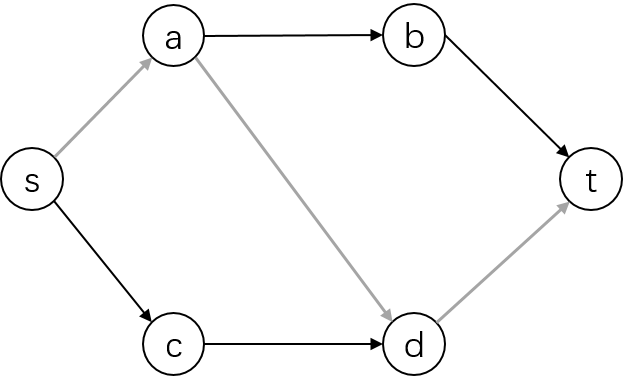
\includegraphics[scale=0.5]{figures/blocking-flow.png}
      \caption{阻塞流非最大流的一个例子。黑色边是非饱和边,灰色边是饱和边}
      \label{Fig:blocking-flow}
  \end{figure}

  下面考虑如何构造阻塞流。前面已经提到,分层图$G'_f$是一个流网络;所以一个自然的想法便是在$G'_f$上不断地DFS寻找增广路\footnote{准确地说应该是「在$G'_f$的残量网络上找增广路」,但我们在$G'_f$要求的是一个阻塞流而不是最大流,无须考虑反向边。}并沿着找到的增广路增广。每次增广至少会使一条边饱和,所以至多增广$m$次;可以在$O(m)$的时间内在分层图上找到一条$s\leadsto t$增广路。,所以构造阻塞流的复杂度不超过$O(m^2)$。下面我们介绍一种称作「当前边」的优化\footnote{有的资料将此优化称作当前弧优化},可使构造阻塞流的复杂度达到$O(nm)$。另外还有一个称作「多路增广」的实现技巧,可进一步优化时间复杂度。
  \subsubsection*{当前边优化}
  对分层图中的每个节点$u$维护一个当前边,初始时初始时$u$的当前边为$u$的邻接边表中的第一条边。每次DFS到点$u$时,从$u$的当前边,设为$(u,v)$,向下递归。若DFS($v$)未找到从$v$到汇点$t$ 的路径,就把$u$的当前边变为$u$的邻接边表中的下一条边,这相当于将边$(u,v)$从分层图中删除;若找到了到$t$的路径就一路回溯。

  我们来分析这种方法构造阻塞流的复杂度。整个过程的复杂度可以化归为调用DFS($v$)的次数。若DFS($v$)的返回值为「找到了路径」则这种调用以$l$个为一组($l$为分层图的层数),每次找到一条$s\leadsto t$路径至少使一条边饱和,这种调用至多有$lm\le nm$次\footnote{残量网络$G_f$中最多有$2m$条边,但是边$(u,v)$和边$(v,u)$不可能同时出现在分层图$G'_f$中,所以$G'_f$中至多有$m$条边。}。若DFS($v$)的返回值为「未找到路径」则有一条边被删除,故这种调用不超过$m$次。所以构造阻塞流的复杂度为$O(nm)$。
  \subsubsection*{多路增广}
  用$c_f(v)$表示DFS到$v$点时从$s$到$v$所经过的边的残余容量的最小值,$c_f(s) = \infty$。
  多路增广是指DFS到$t$点后不一直向上回溯到源点$s$,而是一旦回溯到$c_f(v)>0$的点$v$就从$v$继续向下递归。这里所说的「一旦回溯到$c_f(v)>0$的点$v$」也就是找到的$s\leadsto t$增广路上距离$s$点最近的\emph{饱和边}的起点。把$c_f(v)$也作为DFS的参数,即调用DFS($v$, $c_f(v)$)。当$c_f(v)$变为$0$时就终止DFS($v$, $c_f(v)$)过程。

  \subsubsection*{小结}
  借助分层图这一概念,我们可以很直观地理解引理 \ref{Lemma:1}。Dinic算法的过程就是不断的构造阻塞流,并用阻塞流来增广原来的流$f$;不难看出每次用阻塞流增广$f$之后,残量网络上的最短$s\leadsto t$路径的长度严格递增,所以Dinic算法最多构造$n-1$次阻塞流,因而复杂度为$O(n^2m)$。此复杂度上界是比较松的,Dinic算法的速度能满足大部分实际问题的要求。

  %(由于$G'_f$是$G_f$的子图,将$G'_f$上$s\leadsto t$路径称作增广路是不失严格性的)

  \subsection{ISAP算法}
  ISAP是Improved Shortest Augmenting Path的缩写,ISAP算法来源于R. K. Ahuja,T. L. Magnanti和J. B. Orlin三人合著的\emph{Network Flows: Theory, Algorithms, and Applications}一书的\S 7.4 shortest augmenting path algorithm中提到的对SAP算法的一个优化。在介绍此优化方法之前,我们先介绍SAP算法。顾名思义,SAP算法也是一种最短增广路算法;SAP算法中引入了一些新概念,下面一一介绍。
  \subsubsection*{距离标号}
  设$G(V,E,c,s,t)$是一个流网络,$f$是$G$上的一个流。在残量网络$G_f=(V,E_f)$上,我们定义一个距离函数$d\colon V\to\mathbb{N}$。若函数$d$满足下面两个条件,则称$d$为合法的距离函数:
  \begin{enumerate}
      \item $d(t) = 0$;
      \item $\forall (u,v)\in E_f, d(u) \le d(v) +1$.
  \end{enumerate}
  我们把$d(u)$称作节点$u$的\emph{距离标号},上述两条件称作合法条件。
  \begin{property}
    若距离函数$d$合法,设$p$是残量网络$G_f$上的$u\leadsto t$路径,则$p$上的点的距离标号的集合由从零开始的若干连续自然数组成。
  \end{property}
  \begin{property}\label{P:lower_bound}
      若距离函数$d$合法,则距离标号$d(u)$是残量网络$G_f$上从$u$到$t$的距离的一个下界。
  \end{property}
  令$v=v_0\to v_1 \to\dots\to v_{k-1}\to v_k$为$G_f$上任意一条从$v$到$t$的长为$k$的路径。合法条件蕴含着
  \begin{align*}
      d(v_{k-1})&\le d(v_k)+1 = d(t)+1=1,\\
      d(v_{k-2})&\le d(v_{k-1})+1\le 2,\\
       &\vdots\\
      d(v) = d(v_0)&\le d(v_1) + 1 \le k.
  \end{align*}
  \begin{property}
      若$d(s)\ge n$则残余网络$G_f$中没有从源点$s$到汇点$t$的路径。
  \end{property}
  由于$d(s)$是$G_f$上从$s$到$t$的距离的一个下界,又$\delta_f(s,t)\le n-1$,所以$d(s)\ge n$意味着$G_f$上不存在$s\leadsto t$路径。

  若对每个点$u\in V$都有$\delta_f(u,t)=d(u)$,则称距离标记是准确的。
  \subsubsection*{允许边和允许路径}
  若边$(u,v)\in E_f$满足$d(u)=d(v)+1$则称$(u,v)$为\emph{允许边},否则称为非允许边。若$G_f$的一条$s\leadsto t$路径$p$完全由可行边构成,则称$p$为\emph{允许路径}。显然有
  \begin{property}
    可行路径是一条最短增广路。
  \end{property}

  \subsubsection*{SAP算法}
  SAP算法的思想与Dinic算法类似\footnote{这里所谓「类似」是指level($u$)与$d(u)$的意义有相似之处;但仍应注意分层图$G'_f$上的边和残余网络$G_f$中的可行边这两个概念的区别:若令$d(u)=\mathrm{level}(u)$,则分层图上的边一定是可行边;反过来不成立。}。确定一个初始的合法距离标号,SAP算法重复「DFS找可行路径」的过程,直到残量网络上不存在$s\leadsto t$路径。DFS由前进(advance)、后退(retreat)和重标号(relabel)三种操作构成,详述如下:

  从$s$开始,沿着允许边走,试图到达$t$;若能到达$t$,则沿着找到的最短增广路增广,在新的残量网络上继续寻找允许路径。与Dinic算法不同的是,若走到$u$点之后无法继续\emph{前进},即没有以$u$为起点的可行边,则将$d(u)$增大为$\min\{d(v)+1\colon (u,v)\in E_f\}$,这一操作称作\emph{重标号};然后\emph{后退}一步继续寻找可行边。上述DFS过程采用递归实现比较方便,但顾及效率,下面我们给出SAP算法的迭代实现。在迭代实现中,我们需要维护(i)每个点的「当前边」,点$u$的当前边是指走到$u$时要选择的那条出边;(ii)当前找到的「部分可行路径」。
  \lstinputlisting{code/sap.cpp}
  %DFS走过一条允许边称作\emph{前进}(advance);回溯一步称作\emph{回退}(retreat)。
  \subsubsection{SAP算法的正确性}
  不难验证:(i)重标号操作使一个点的距离标号严格增大;(ii)增广和重标号这两种操作能维持距离标号的合法性。再结合性质\ref{P:lower_bound},可以推出:(i) SAP算法能在有限次重标号操作之后找到一条最短增广路;(ii) SAP算法能在有限次重标号和增广之后求出一个最大流。
  %要证明SAP算法的正确性只要证明增广和重标号这两种操作能保证距离标号的合法性。首先,不难看出重标号操作使一个点的距离标号严格增大。先考虑增广操作,设边$(u,v)$在SAP算法找到的某条增广路上,若$(v,u)$是增广之后新出现在残量网络上的边,$d(u)\le d(v)+1$蕴含着$d(v)\le d(u)+1$。再考虑重标号操作,我们只要证明在重标号操作修改了$d(u)$之后,$u$的所有入边仍是允许边($u$的所有出边在重标号之后显然仍满足合法条件)。
  \subsubsection{SAP算法的复杂度}
  SAP算法的复杂度可分成四部分考虑:
  \begin{enumerate}
    \item 检查点的出边是否为允许边
    \item 重标号
    \item 前进和后退的总次数
    \item 增广
  \end{enumerate}

  注意到(i)对点$u$重标号的前提是遍历$u$的出边而未找到允许边;(ii)对$u$重标号的复杂度即遍历$u$的出边的复杂度。所以重标号的总复杂度不超过检查点的出边是否为允许边的复杂度。我们可以得出
  \begin{property}
    若SAP算法对每个点重标号不超过$k$次,则「检查点的出边是否为允许边」和「计算新距离标号」的总复杂度为$O(k\sum\limits_{u\in V}|E(u)|)=O(km)$。其中$E(u)=\{(v,w)\in E\colon v= u \text{ 或}\ w = u\}$。
  \end{property}
  另外注意到,每次对点$u$重标号之前我们已经找到了一条完全由允许边组成的$s\leadsto u$路径,从而有$d(u)\le d(s)< n$;又重标号之后$d(u)$至少增加$1$,所以$u$经历过至多$n$次重标号。因此(i)重标号的总次数为$O(n^2)$,后退的总次数也是$O(n^2)$;(ii)寻找允许边和计算新距离标号的总复杂度为$O(nm)$。

  再考虑增广的总复杂度。采用定理\ref{T:number-of-augmentations} 的证明思路,我们可以证明:
  \begin{theorem}
    SAP算法的增广次数为$O(nm)$。
  \end{theorem}
  因为一次增广的复杂度为$O(n)$,故增广的总复杂度为$O(n^2m)$,从而前进的总次数为$O(n^2m+n^2)=O(n^2m)$。综上所述,SAP算法的复杂度为$O(n^2m)$。
  \subsubsection{优化}
  SAP算法终止的条件是$d(s)\ge n$,但实际中往往在$d(s)\ge n$达成之前很久就已经算出一个最大流了。在最大流求出之后进行的种种操作显然是多余的,下面我们要介绍的优化能及时检测到当前残量网络上出现了一个最小割亦即求得了一个最大流。

  维护一个长为$n$的数组num,num[$i$]表示当前残量网络上距离标号为$i$的点的数目($0\le i < n$)。初始的合法距离标号不能任意设置,需要保证num数组中的非零项连续,亦即存在某个下标$l$使得$\mathrm{num}[0],\mathrm{num}[1],\dots,\mathrm{num}[l]$都大于零,数组中其他项都为零。要满足这一条件至少有两个选择:(i)所有距离标号都置为$0$;(ii)从$t$点开始反向BFS,求出准确距离标号。每次将某点的距离标号从$k_1$提高到$k_2$,num[$k_1$]减一,num[$k_2$]加一;若num[$k_1$]变为零则终止算法。

  下面来证明此优化的正确性。设num[$k_1$]减为零时求得的流为$f$。令$S=\{v\in V\colon d(v)>k_1\}$,$T=\bar{S}=\{v\in V\colon d(v)<k_1\}$;不难验证$s\in S$,$t\in T$;即$(S,T)$是流网络$G=(V,E)$的一个割。我们将证明$|f|=c(S,T)$。考虑点对$u\in S$和$v\in T$,由$S$和$T$的定义可知$d(u)>d(v)+1$,所以$(u,v)\notin E_f$。由$(u,v)\notin E_f$可推出(i)若$(u,v)\in E$则必有$f(u,v) = c(u,v)$;(ii)若$(v,u)\in E$则必有$f(v,u)=0$。因此我们有
  \begin{align*}
    f(S,T) &= \sum_{u\in S}\sum_{v\in T}f(u,v)-\sum_{v\in T}\sum_{u\in S}f(v,u)\\
    &= \sum_{u\in S}\sum_{v\in T}c(u,v)-\sum_{v\in T}\sum_{u\in S}0\\
    &= c(S,T)
  \end{align*}
  所以$|f|=f(S,T)=c(S,T)$。% TODO  证明可简化

  下面给出ISAP算法的代码,我们采用逆向BFS求每个点的准确距离标号,其中\texttt{augment}函数与SAP算法中相同,略去。
  \lstinputlisting{code/isap.cpp}
  \subsection{网络流的建图}
  网络流问题包括最大流的费用流两大类,这一小节我们只考虑最大流的建图(或称建模)。最大流的建图一般从流和割两个角度考虑。
  \subsubsection{从流的角度建图}
  从流的角度考虑,一般的思路是:将某种操作看做从源点经若干个中间点推送一定数量的流到汇点,这些流量经过边的容量表示对这种操作做出的种种限制。下面给出一个例子。
  \begin{example}[Collector's Problem, UVa 10779]
    Bob和朋友们在收集糖果中的贴纸。为了让自己手中的贴纸种类尽量多,他们决定用一张重复的贴纸去和别人交换一张自己所没有的贴纸。Bob意识到只跟别人交换自己所没有的贴纸并不总是最优的,在某些情况下,换来一张已有的贴纸更划算。
    假设Bob的朋友们只跟Bob交换贴纸(他们之间不交换),并且这些朋友只拿自己重复的贴纸去跟Bob交换自己所没有贴纸。试问Bob最多能获得多少种贴纸?
  \end{example}
  建图方式:用点$a_i$表示第$i$种贴纸,设Bob有$c_i$张这种贴纸,从源点$s$向$a_i$连一条容量为$c_i$的边,从$a_i$向汇点$t$连一条容量为$1$的边。
  用点$b_j$表示Bob的第$j$个朋友。若朋友$j$没有第$i$种贴纸,就从$a_i$向$b_j$连一条容量为$1$的边;若朋友$j$有$k$($k\ge 2$)张第$i$种贴纸,就从$b_j$向$a_i$连一条容量为$k-1$的边。不难证明,最大流的值便是Bob所能获得的贴纸种类的最大值。
  \subsubsection*{从割的角度建图}
  从割的角度考虑,通常的思路是用有向边表示一个二元关系,我们要在满足一组二元关系的条件下求解一个最优化问题。下面以有向图的\emph{最大权闭包}(maximum weight closure)问题为例,介绍最小割建模。
  \begin{example}[最大权闭包]
  设$G=(V,E)$是一个有向图,若$V_1\subseteq V$满足:$\forall (u,v) \in E$,$u\in V_1 \Rightarrow v\in V_1$,则称$V_1$是$G$的一个闭包,图\ref{Fig:closure} 给出了一个例子。给图$G$每个节点$u$赋一个权值$w(u)\in \mathbb{Z}$,点集$X\subseteq V$的权值$w(X)$定义为$w(X)=\sum_{v\in X}w(v)$;最大权闭包问题即,求$G$的一个权值最大的闭包。
  \begin{figure}
    \centering
    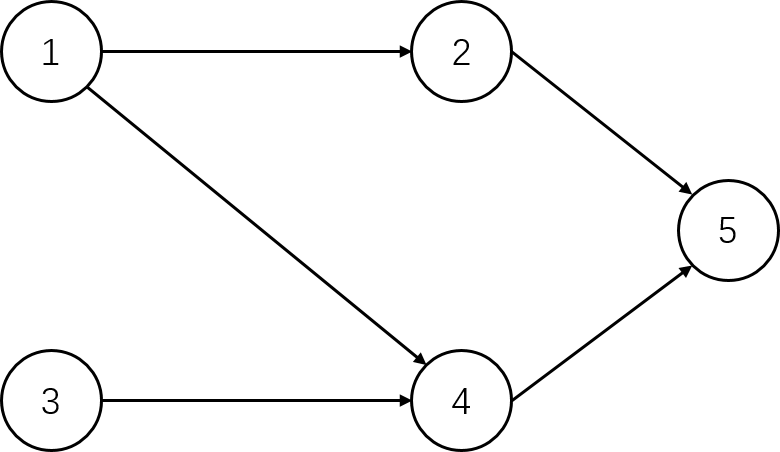
\includegraphics[scale=0.4]{figures/closure}
    \caption{有向图的闭包。$\{2,5\}$,$\{1,2,4,5\}$,$\{3,4,5\}$都是闭包。}
    \label{Fig:closure}
  \end{figure}
\end{example}
  我们可以将最大权闭包问题转化成最小割问题。引入源点$s$和汇点$t$,从$s$向每个权值为正的点$u$连一条容量为$w(u)$的边,从每个权值为负的点$u$向$t$连一条容量为$-w(u)$的边,将原图中的边的容量设为$\infty$(这里,$\infty$是指一个大于$\sum_{v\in V}|w(v)|$的值)。将所得流网络记做$G'=(V',E')$。

  设$(S,T)$是网络$G'$的一个割。若$(S,T)$的任意前项边$(u,v)$都满足$u\in S$或$v\in T$,则称$(S,T)$为\emph{简单割}(simple cut)。不难证明,有向图$G$的闭包和网络$G'$的简单割一一对应。读者可自行验证,(i)若$V_1$是$G$的一个闭包,令$S=\{s\}\cup V_1$,则$(S,\bar{S})$是$G'$的一个简单割;(ii)若$(S,\bar{S})$是$G'$的一个简单割,令$V_1=S-s$,则$V_1$是$G$的一个闭包。
  \begin{figure}
    \centering
    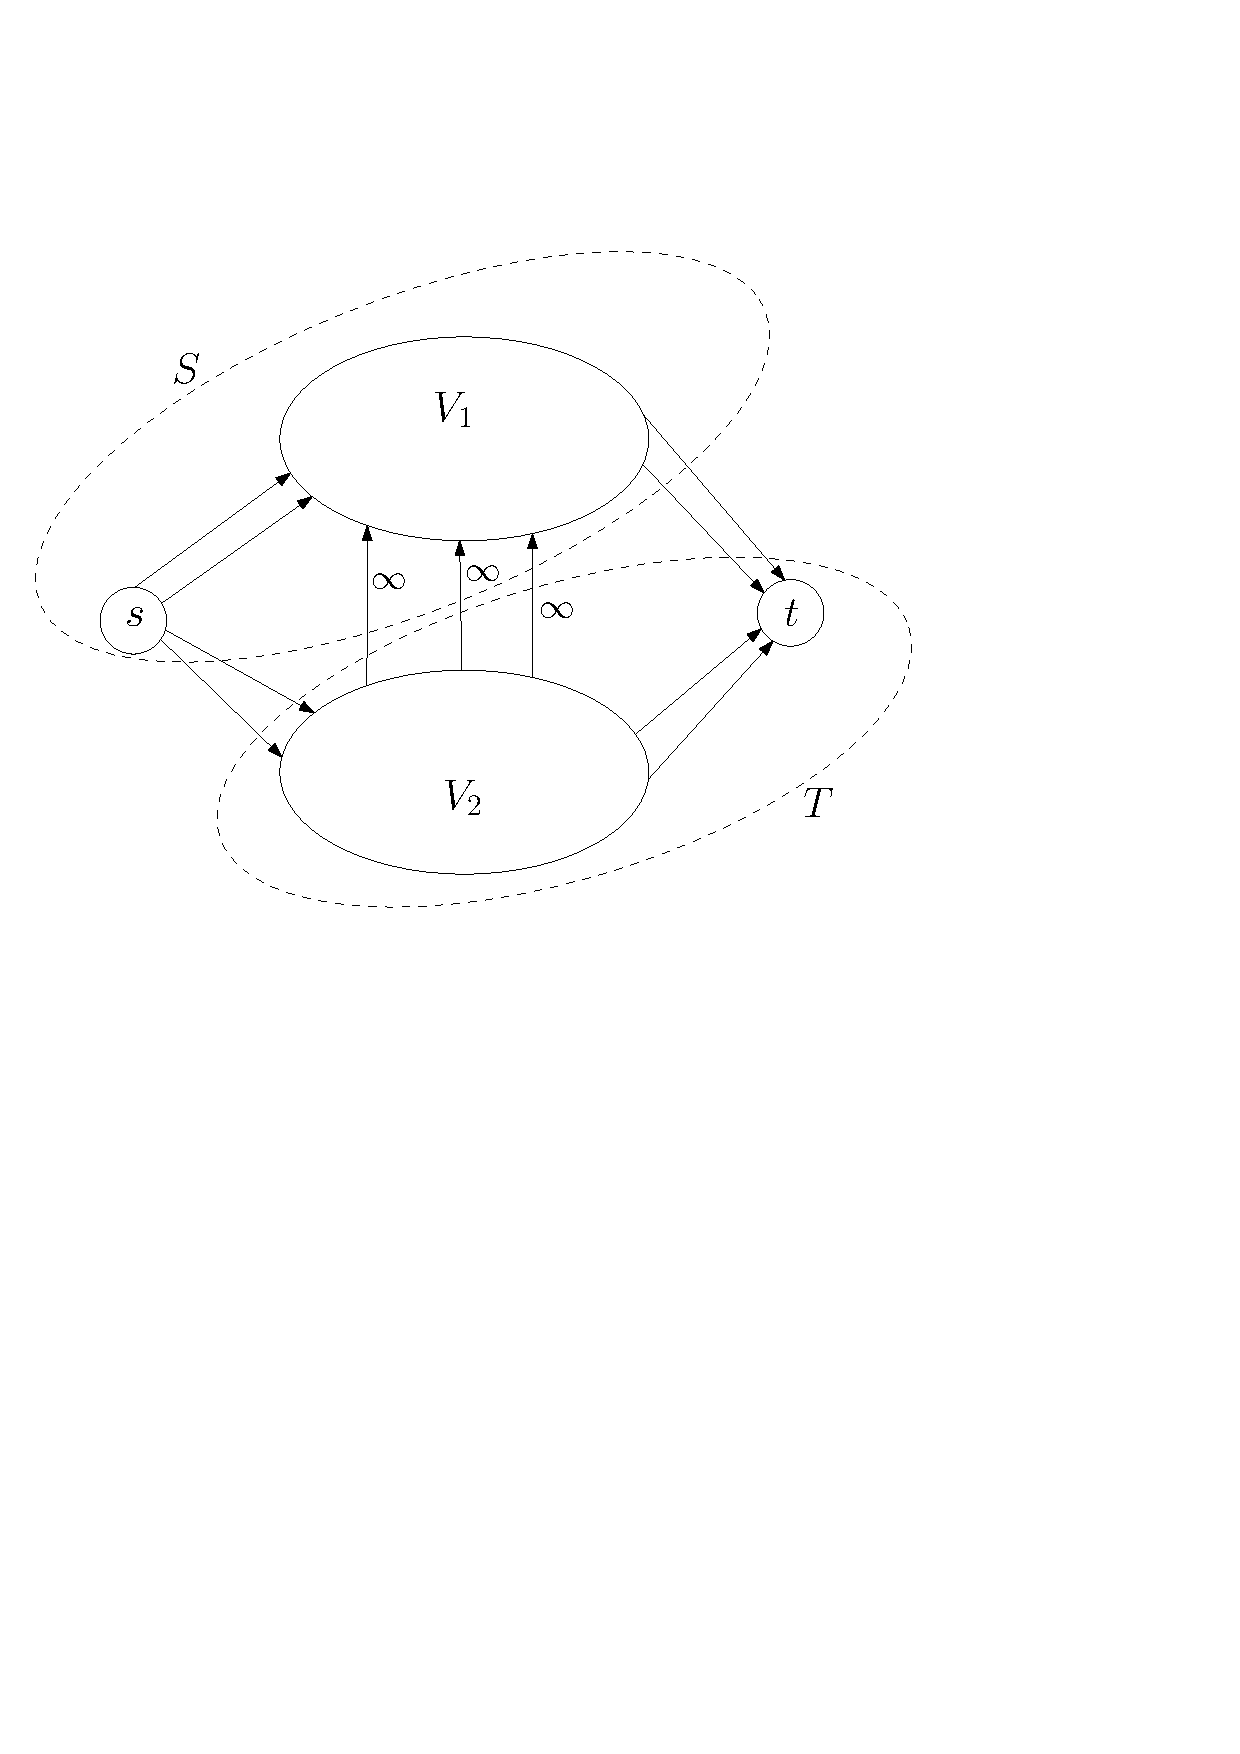
\includegraphics[scale=0.5]{figures/simple-cut}
    \caption{简单割示意。}
    \label{Fig:simple-cut}
  \end{figure}
  我们来考虑简单割$(S,\bar{S})$的容量$c(S,\bar{S})$和$G$的闭包$V_1=S-s$的权值$w(V_1)$之间的关系。如图\ref{Fig:simple-cut} 所示,设$V_1$中权值为正的点的集合为$V_1^+$,权值为负的点的集合为$V_1^-$,令$V_2=V-V_1$,类似地定义$V_2^+$、$V_2^-$;我们有
  \begin{align*}
    w(V_1) &=w(V_1^+) + w(V_1^-)\\
    c(S,T) &= \sum_{u\in V_2^+}c(s,u) + \sum_{u\in V_1^-}c(u,t)\\
    % &= \sum_{u\in V_2^+}w(u) - \sum_{u\in V_1^-}w(u)
    &= w(V_2^+) - w(V_1^-)
  \end{align*}
  从而
  \[ w(V_1) + c(S,T) = w(V_1^+) + w(V_2^+) = w(V^+)= \mathrm{const}\]
  其中,$V^+$表示$V$中权值为正的点的集合;$w(V_1)$最大即$c(S,T)$最小,又图$G$中的边的容量都为$\infty$,故$G'$的最小割一定是简单割;这样我们就把最大权闭包问题转化成了最小割问题。
  \section{最小费用流}
  在最大流问题的基础上,我们来讨论另一个网络流问题---\emph{最小费用流}(minimum cost flow)问题。在最小费用流问题中,边$(u,v)\in E$除了有容量$c(u,v)$之外还有\emph{费用}$\cost(u,v)\in\mathbb{N}$,表示单位流量流过$(u,v)$的花费。给定流$f$,边$(u,v)$上产生的费用为$\cost(u,v) f(u,v)$,流$f$的费用$\cost(f)$定义为$\cost(f) = \sum_{(u,v)\in E}\cost(u,v)f(u,v)$。最小费用流问题有三种常见的形式:
  \begin{enumerate}
    \item 给定费用流网络$G=(V,E,s,t,c,\cost)$,求费用最小的最大流。
    \item 给定费用流网络$G=(V,E,s,t,c,\cost)$,求一个值为$x$且费用最小的流。
    \item 最小费用流问题的一般形式。不再区别源点与汇点,每个点$v\in V$都关联了一个值$b(v)\in\mathbb{Z}$,$b(v)>0$代表\emph{供给}(supply),$b(v)<0$代表\emph{需求}(demand)。我们要求一个流$f$使其满足(i)边的容量限制;(ii)点的供需要求;(iii)费用最小。形式化地写成
    \begin{equation}
      \min\sum_{{u,v}\in E}\cost(u,v)f(u,v), \label{mcf-obj}
    \end{equation}
    subject to
    \begin{align}
      \sum_{v\colon(u,v)\in E} f(u,v) &- \sum_{v\colon(v,u)\in E}f(v,u) = b(u) \quad \forall u\in V,\label{Ineq:capacity}\\
      0\le f(u,v)&\le c(u,v)\quad \forall(u,v)\in E\label{Eq:balance} %TODO 让两个公式都居中
    \end{align}
    把满足 \eqref{Ineq:capacity} 和 \eqref{Eq:balance} 的流称作\emph{可行流}。
  \end{enumerate}
  不难证明,这三种形式是等价的。下面我们只讨论\emph{最小费用最大流}(min-cost max-flow)问题。

  我们仍然采用增广路方法来求解。
  不难看出,若$(u,v)\in E$且$(u,v)\in E_f$,那么在残量网络$G_f$上,边$(v,u)$的费用$\cost(v,u)$应为$-\cost(u,v)$。容易想到一个贪心策略:把边的费用视作距离,在$G_f$上总是沿着最短增广路增广。这个想法是正确的,证明从略。% TODO 补上证明
  此算法称作\emph{连续最短路算法}(successive shortest path algorithm)。
  % FIXME 坚持原创 ^-^
  由于可能有负权边,不能用Dijkstra算法求最短路,而用Bellman-Ford算法。
  下面给出代码,图的表示与前面介绍的最大流算法的相比只多出了费用\texttt{cost},\texttt{add\_edge}函数也要做相应的修改,略去不表。
  \lstinputlisting{code/mcmf.cpp}
  %\section{dummy}
  \section{二分图}
  二分图是一类特殊的无向图,其点集$V$可划分为两个不相交的子集$L$和$R$使得$E$中每条边的端点分属$L$、$R$。形式化地说,无向图$G=(V,E)$是二分图,当且仅当存在点集$V$的\emph{二划分}(bipartition)$\{L,R\}$使得$E\subseteq L\times R$。二分图也记做$G=(L,R;E)$。
  \begin{figure}
    \centering
    \begin{subfigure}[t]{0.4\linewidth}
      \centering
      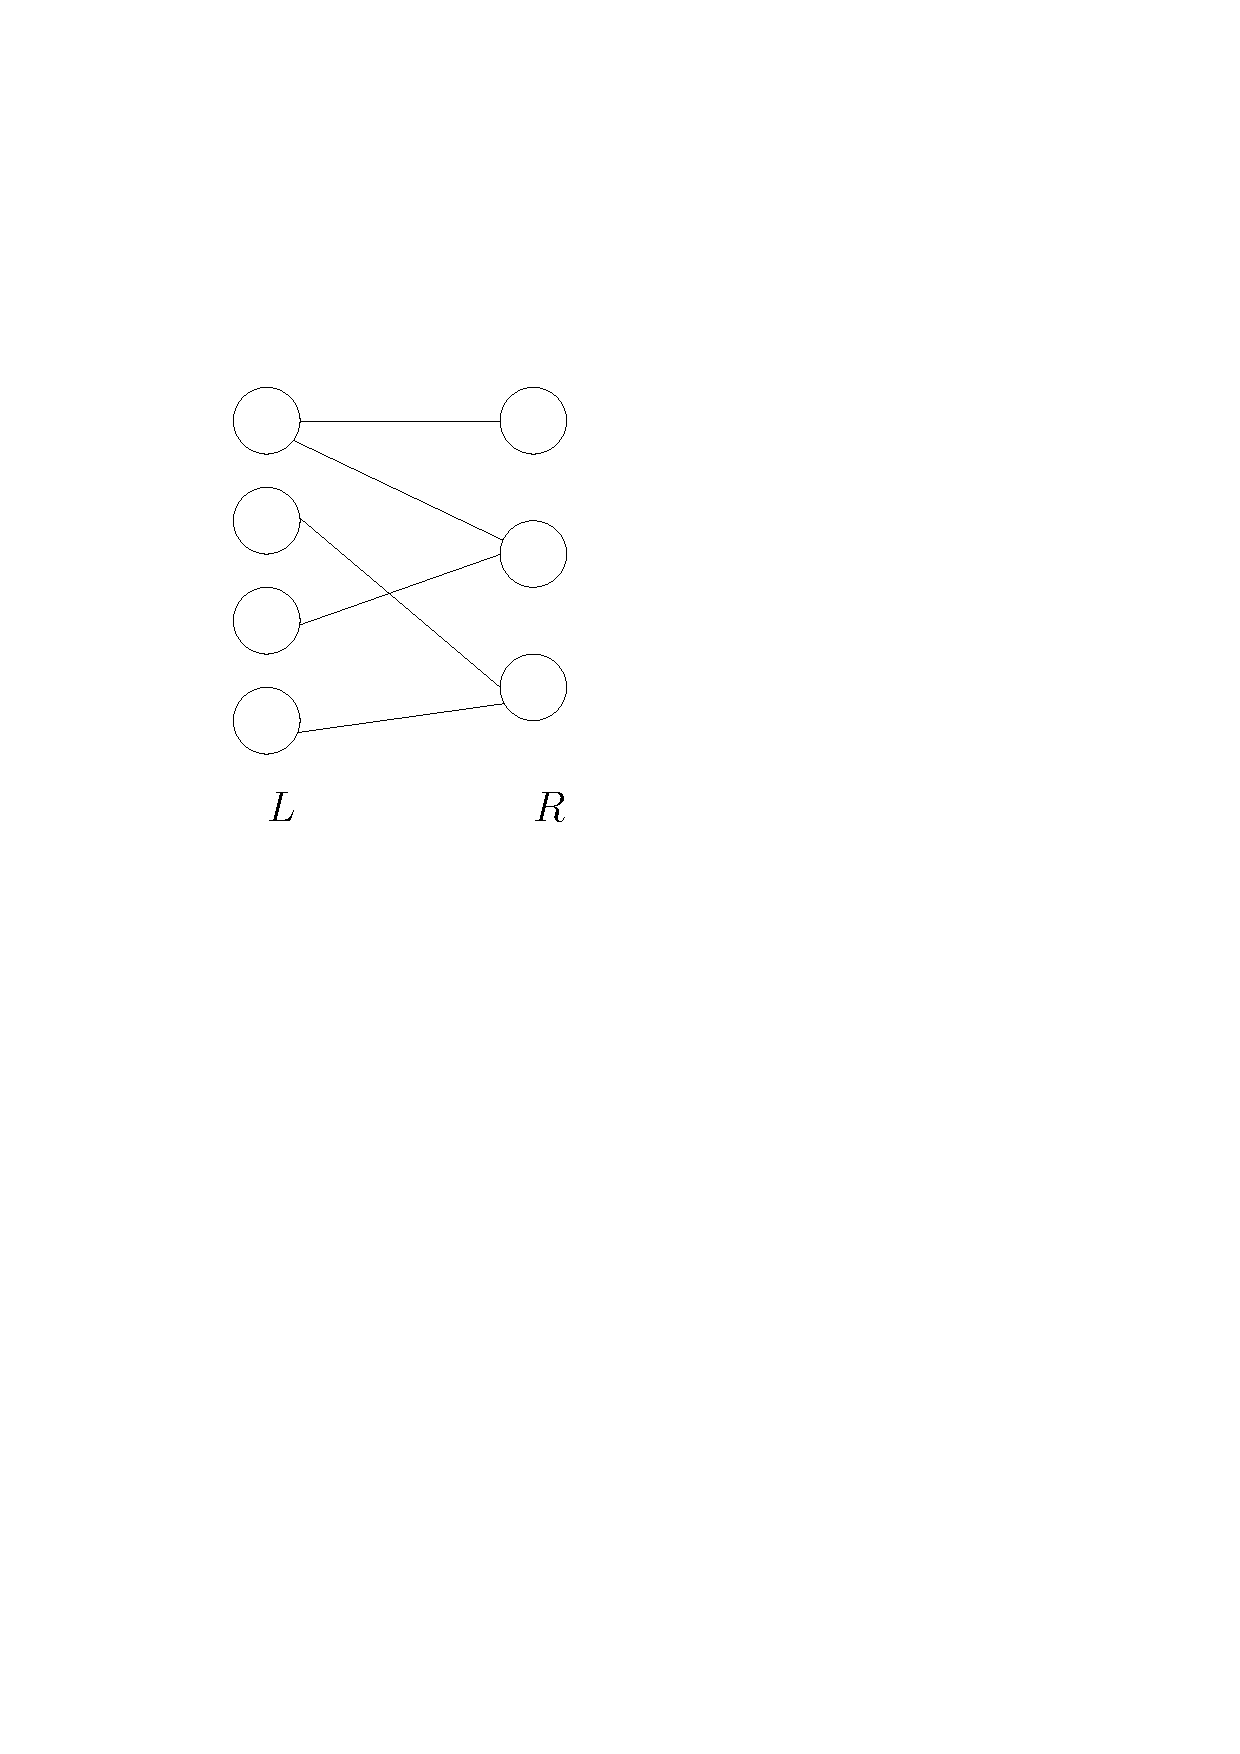
\includegraphics[scale=0.5]{figures/bipartite-graph}
      \caption{}
      % \label{Fig:bipartite}
    \end{subfigure}
    \begin{subfigure}[t]{0.4\linewidth}
      \centering
      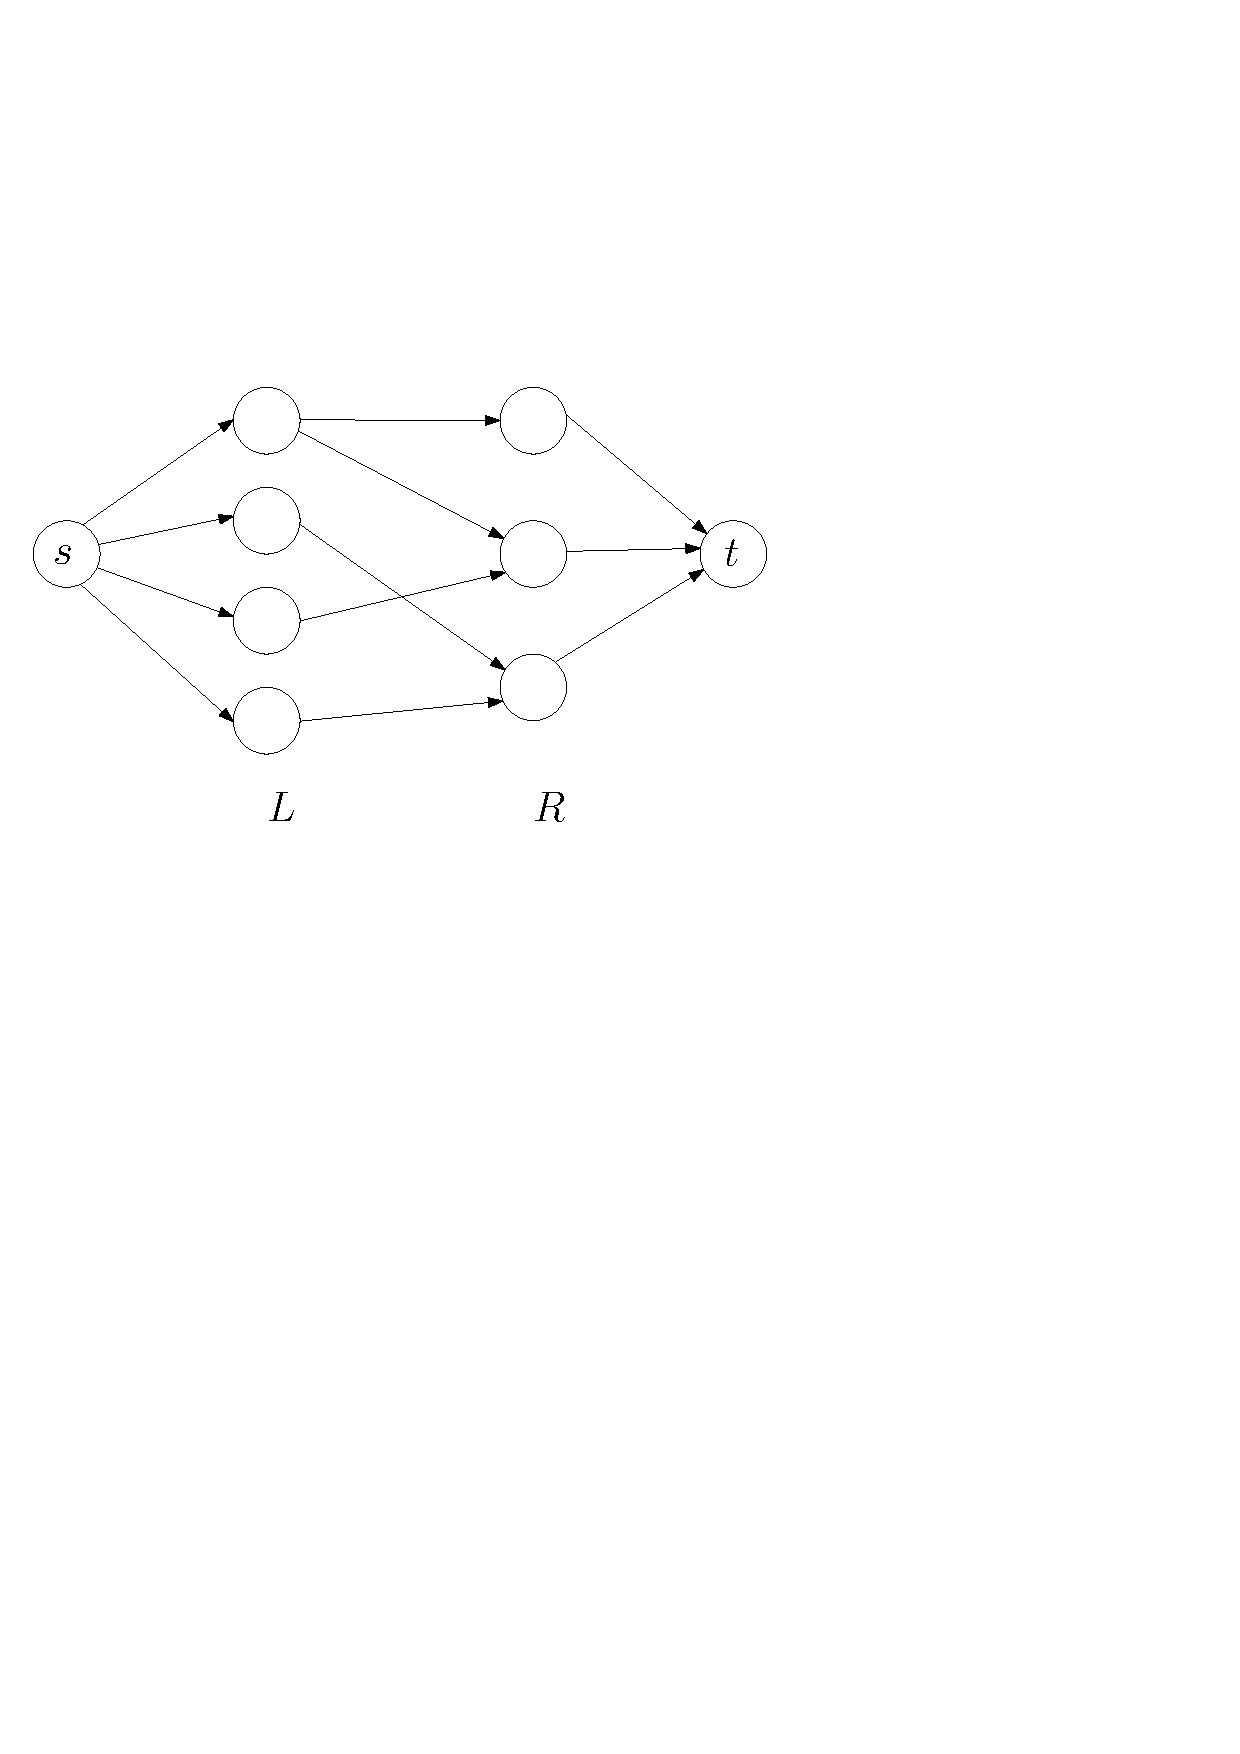
\includegraphics[scale=0.5]{figures/bipartite-network}
      \caption{}
    \end{subfigure}
    \caption{二分图和对应的流网络。}
    \label{Fig:bipartite-network}
  \end{figure}
  \subsection{二分图的最大匹配}
  在这一小节我们用最大流模型来解决\emph{二分图最大匹配}(maximum bipartite matching)问题。
  \subsubsection*{无向图的匹配}
  设$G=(V,E)$是一个无向图,若边集$M\subseteq E$满足:对任意节点$v\in V$,$M$中至多有一条边以$v$为端点则称$M$是$G$上的一个\emph{匹配}(matching)。若$v\in V$是$M$中某条边的端点,则称$v$是$M$上的匹配点,否则称为非匹配点。$M$中的边称为匹配边,$E-M$中的边称为非匹配边。最大匹配即边数最大的一个匹配。若图$G$的所有顶点都是匹配点,则称$M$为\emph{完美匹配}(perfect matching)。显然,完美匹配存在的前提是$|V|$为偶数。
  \subsubsection{二分图的最大匹配与最大流}
  二分图的最大匹配问题可以转化为最大流问题。如图\ref{Fig:bipartite-network} 所示,给定二分图$G(V,E)$,$V=L\cup R$,我们可以构造一个流网络$G'=(V',E')$:
  \begin{align*}
    V'&=V\cup\{s,t\},\\
    E'&=\{(s,u)\colon u\in L\}\cup\{(u,v)\colon(u,v)\in E\}\cup\{(v,t)\colon v\in R\}.
  \end{align*}
  将$E'$中每条边的容量置为$1$。注意:$E$中的边是无向边而$E'$中的边是有向边。

  不难证明,二分图$G=(V,E)$的最大匹配数等于对应的流网络$G'=(V',E')$上的最大流的值。下面来分析此算法的复杂度,我们已经知道朴素实现的增广路方法的复杂度不超过$O(|f^*|E)$,其中$|f^*|$表示最大流的值。在二分图的最大匹配中我们有(i) $|f^*|\le\min(L,R)=O(V)$;(ii)没有边与之相连的点不用考虑,故$|V|\le 2|E|$,因此$|E'|=|E|+|V|\le3|E|$。故而可以在$O(VE')=O(VE)$的时间内求出二分图$G=(V,E)$的最大匹配。
  \subsection{匈牙利算法}
  \emph{匈牙利算法}(hungarian algorithm)也称Kuhn-Munkres算法(简称KM算法)。匈牙利算法用于求解\emph{二分图最大权匹配}(maximum weighted bipartite matching)问题。
%  \subsubsection*{二分图的完美匹配}
%  令$G=(V,E)$是一个二分图,$\{A,B\}$是其(顶点的)二划分。不失一般性,设$|A|\le|B|$。设$M$为$G$的最大匹配,若$|M|=|A|$则称$M$为$G$上的\emph{完美匹配}(perfect matching)。
  \subsubsection*{带权二分图}
  给二分图$G=(V,E)$的每条边$(u,v)\in E$赋一个权值$w(u,v)\in\mathbb{N}$就得到了\emph{带权二分图}(weighted bipartite graph)。匹配$M$的权值定义匹配边的权值之和,即$w(M)=\sum_{(u,v)\in M}w(u,v)$。二分图最大权匹配问题即,给定带权二分图$G=(V,E)$,$V$的二划分为$\{X,Y\}$,求一个权值最大的匹配$M$。在二分图最大权匹配问题中,不失一般性,(i)通过添加权值为零的边,我们可以假定图$G=(V,E)$是完全二分图,即$\forall u\in L,v\in R,(u,v)\in E$;(ii)通过添加虚拟节点,我们可以假定$|X|=|Y|$,此时我们总可以求出一个权值最大的完美匹配。加上了这两个假定之后的二分图最大权匹配问题也称作二分图最大权完美匹配问题或者\emph{指派问题}(assignment problem)。这小节中,我们在上述两假定下讨论二分图的最大权完美匹配问题。
  \begin{figure}
    \centering
    \begin{subfigure}[t]{0.45\linewidth}
      \centering
      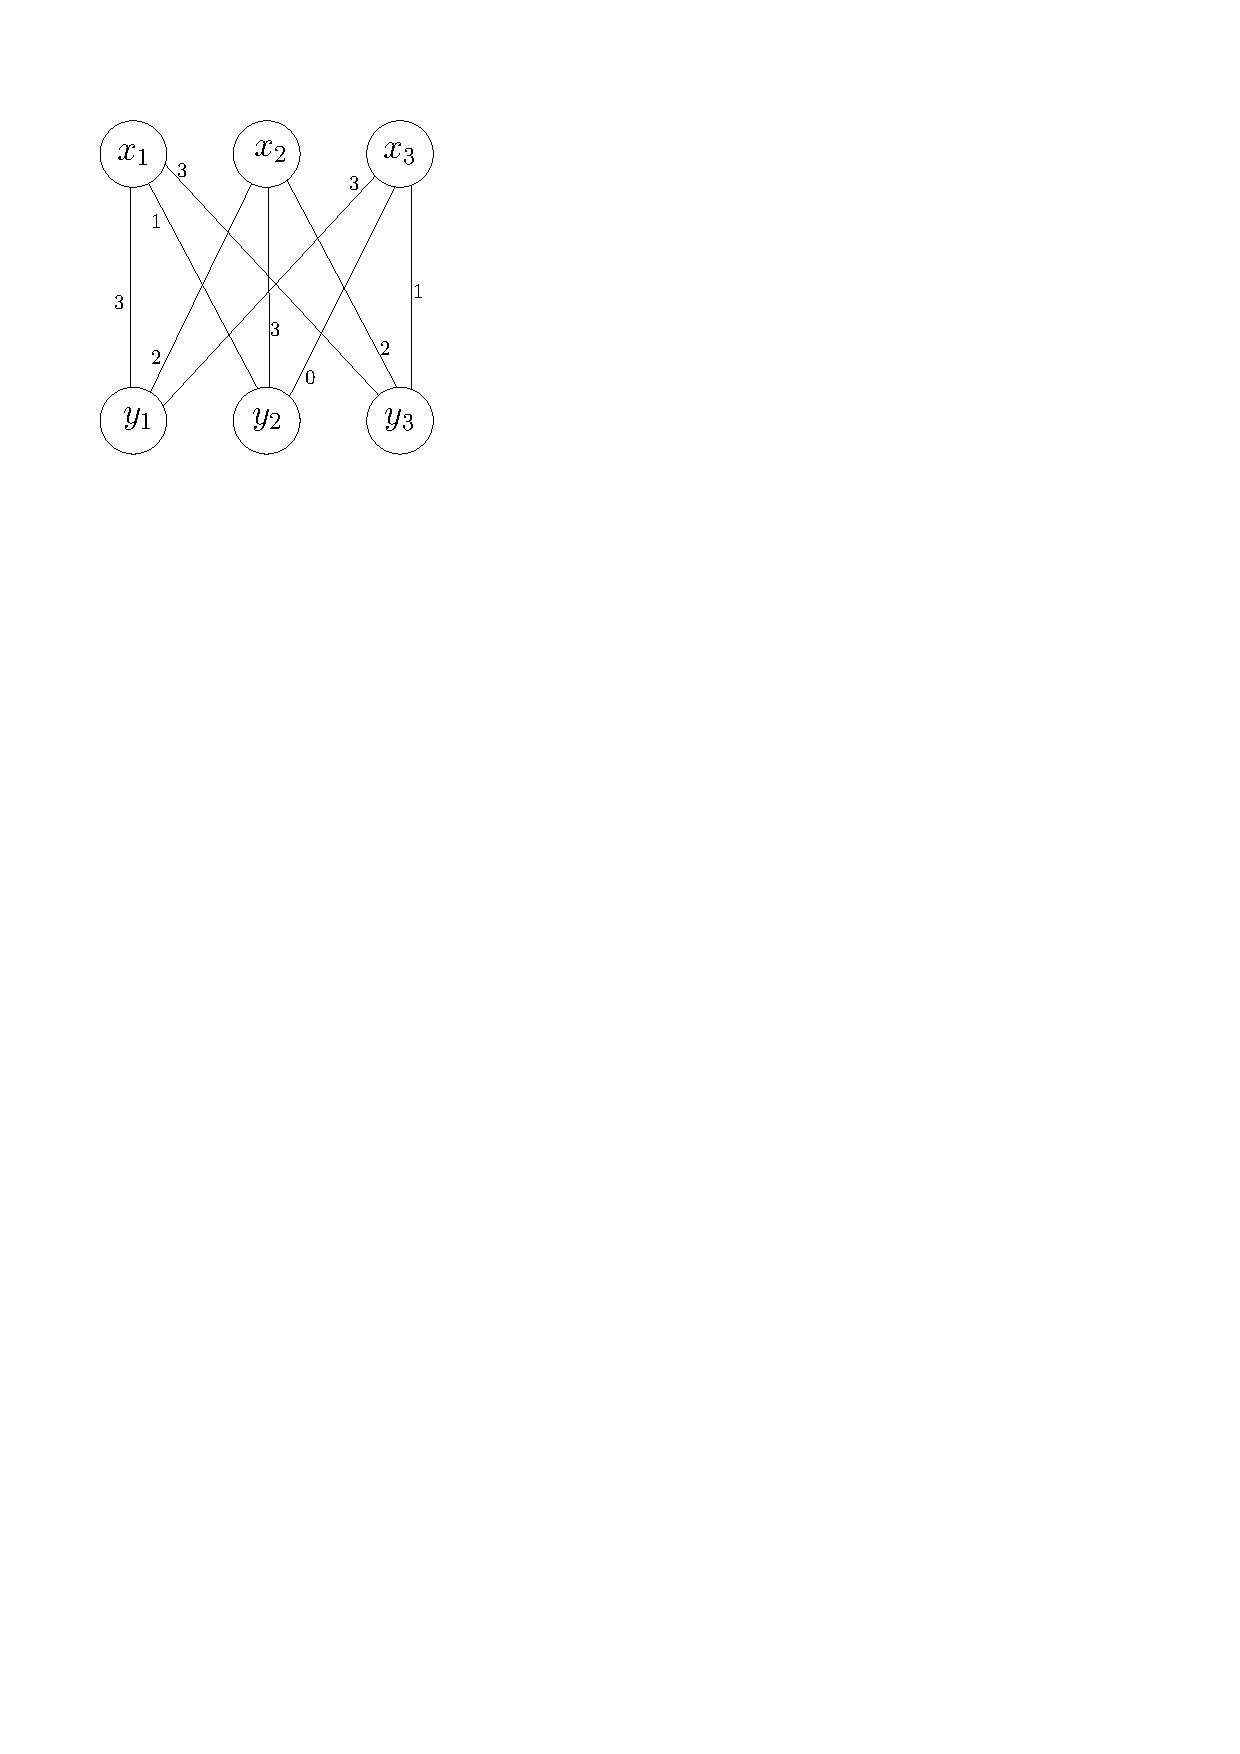
\includegraphics[scale=0.8]{figures/weighted-bipartite}
      \caption{带权完全二分图}
    \end{subfigure}
    \begin{subfigure}[t]{0.45\linewidth}
      \centering
      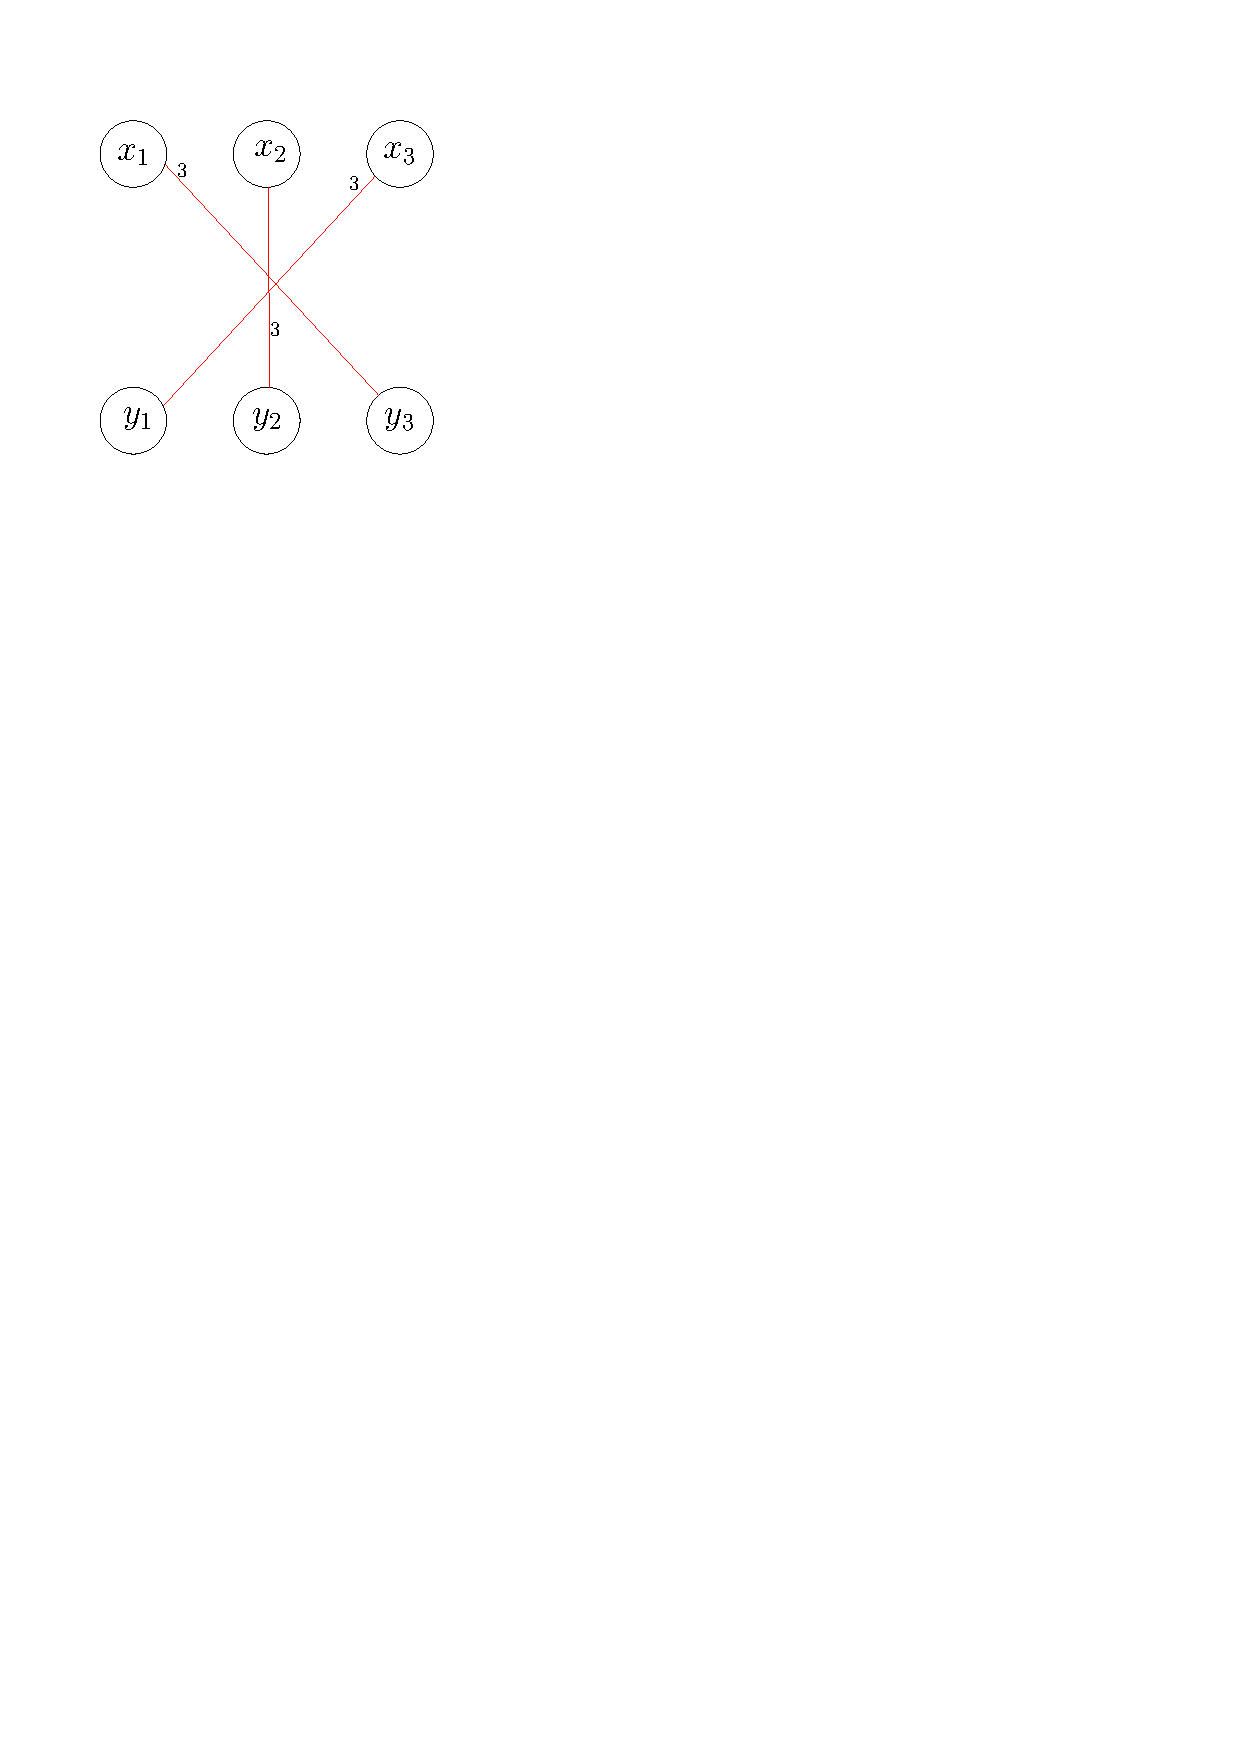
\includegraphics[scale=0.8]{figures/max-weighted-bipartite-match}
      \caption{带权最大匹配}
    \end{subfigure}
    \caption{二分图最大权匹配问题。}
    % \label{}
  \end{figure}
  \subsubsection*{交错路和交错树}
  令$M$为二分图$G=(V,E)$的一个匹配。设$P$为$G$上一条简单路径\footnote{这里我们将路径视作边的集合,故用大写字母$P$表示。},若$P$中的边交替地出现在$M$和$E-M$中则称$M$为\emph{交错路}(alterntating path)\footnote{有的文献中规定交错路至少有一个端点是非匹配点}。若$P$的两端点都是非匹配点,则称$p$为增广路;不难验证,(i)增广路上的非匹配边比匹配边多一条,(ii)将$P$上的匹配边和非匹配边对调,得到的边集$M'$仍是$G$上的一个匹配,且$|M'|=|M|+1$;这正是称$p$为增广路的原因。增广操作可以用\emph{对称差}(symmetric difference,$\oplus$)这一集合运算来表示;设$A$、$B$为两集合,对称差$A\oplus B$定义为$(A-B)\cup(B-A)$,即恰属于这两集合中某一个的元素的集合。我们有$M'=M\oplus P$。

  由$G$和$M$所导出的\emph{交错树}(alternating tree)是一棵有根树,它满足:(i)以某个非匹配点为根,(ii)从根到树中每个节点的路径都是交错路。
  \subsubsection{顶点标号和相等图}
  设$G=(V,E)$是一个二分图,$V$划分为$\{X,Y\}$。顶点标号是一个函数$l\colon V\to\mathbb{R}$。称$l$为可行标号若它满足
  \[
    l(x)+l(y)\ge w(x,y),\quad \forall x\in X, y\in Y.
  \]

  \emph{相等图}(equlity graph)$G_l=(V,E_l)$是由$G$和$l$所导出的一个图,
  \[
    E_l = \{(x,y)\in E\colon l(x)+l(y)=w(x,y)\}.
  \]
  显然有
  \begin{theorem}
    若$l$是一个可行标号函数且$M\subseteq E_l$是一个完美匹配,则$M$是一个最大权匹配。
  \end{theorem}
  下面给出匈牙利算法的伪代码:
  \begin{codebox}
    \Procname{$\proc{Hungarian}(G,w)$}
    \li 令$l$为某一可行标号,$M$为$G_l$上的某个匹配
    \li \While $M$不是完美匹配
    \li \Do \label{li:begin-augment}
          \If $G_l$中不存在$M$的增广路
    \li     \Then
              计算新标号函数$l'$使得$M\subset E_{l'}$且$G_{l'}$上存在$M$的增广路 \label{li:improve-label-1}
    \li       $l \gets l'$
          \End
    \li   在$G_l$上找一条增广路$P$
    \li   $M=M\oplus P$
        \End  \label{li:end-augment}
    \li    \Return $M$
  \end{codebox}
  初始的可行标号可置为
  \[\forall y\in Y,\ l(y)=0,\quad \forall x\in X,\  l(x)=\max_{y\in Y}\{w(x,y)\}.\]
  匈牙利算法的核心是上述伪代码的第\ref{li:improve-label-1}~行,即优化可行标号使得有新边进入相等图且出现增广路。下面讲述如何优化可行标号,为此,先介绍邻集这一概念。

  令$l$是某个可行标号,点$u\in V$在$G_l$上的\emph{邻集}(neighbor)定义为$N_l(u)=\{v\in V\colon(u,v)\in E_l\}$,类似地,点集$S\subseteq V$的邻集定义为$N_l(S)=\bigcup_{u\in S}N_l(u)$。
  \begin{lemma}\label{L:improve-label}
    设$S\subseteq X$满足$T=N_l(S)\ne Y$。令
    \[
      \alpha_l = \min_{x\in S,y\notin T}\{l(x)+l(y)-w(x,y)\}.
    \]
    又令
    \[l'(v) =
    \begin{cases}
      l(v)-a_l &  \text{若$v\in S$;}\\
      l(v)+a_l &  \text{若$v\in T$;}\\
      l(v) & \text{其他情况.}
    \end{cases}
    \]
    则$l'$是一个可行标号且满足
    \begin{enumerate}
      \item 对于$x\in S,y\in T$,若$(x,y)\in E_l$, 则$(x,y)\in E_{l'}$;\label{P:1}
      \item 对于$x\notin S, y\notin T$,若$(x,y)\in E_l$, 则$(x,y)\in E_{l'}$;
      \item 存在边$(x,y)\in E_{l'}$满足$x\in S,y\notin T$。\label{P:3}
    \end{enumerate}
  \end{lemma}
  此引理的正确性几乎是显然的,读者可自行验证。
  %我们要指出,不存在$(x,y)\in E_l$使得$x\in\bar{S},y\in T$;其中$\bar{S}=X-S$。根据邻集的定义,对任意边$(x,y)\in E_l$,$x\in S,y\in N_l(S)=T$和$x\in\bar{S}$
  %匈牙利算法的过程如下:从某个$l$和某个图$G$上某个匹配$M\subset\E_l$开始;若$M$不是$G_l$上的完美匹配,则重复:(i)将$M$增广为$G_l$上的最大匹配,(ii)
  下面我们来考虑怎样选择$S$可以使得按引理\ref{L:improve-label} 得到$E_{l'}$满足(i)$M\subset E_l$且(ii) $E_{l'}$中包含$M$的增广路。为了便于表述,我们定义一个记号,设$S\subseteq V$,$S$的匹配集$\match(S)$定义为
  \[\match(S)=\{t\in V\colon\text{存在}\ s\in S\ \text{使得}\ (s,t)\in M\}\]
  % 在不至引起混淆的情况下,也用$u$表示单元集$\{u\}$。

  我们的思路是利用引理\ref{L:improve-label} 中的$l'$所满足的三条性质,$S$首先要满足$N_l(S)\ne Y$,这样才能利用性质\ref{P:3};因此,
  (i)令$S_0=\{u\}$,$u$是$X$中任意一个未匹配点,由于$M$不是完美匹配,$u$总是存在的;
  (ii)从而$N_l(S_0)$中都是匹配点,为了保证$N_l(S_0)$覆盖的匹配边仍在$E_{l'}$中,根据性质\ref{P:1},再令$S_1=S_0\cup\match(N_l(S_0))$,显然有$S_1\subseteq{X}$;如此反复,直到$\match(N_l(S_k))\subset S_k$。此$S_k$即为所求的$S$。不难看出上述过程是一个不断扩展以$u$为根的交错树的过程。由于$G_l$中不存在增广路所以对任意$1\le i\le k$,$N_l(S_i)$中全是匹配点,从而有$N_l(S_i)\ne Y$。因此$S_k$即为我们所要求的$S$。

  由上述分析可知$N_l(S)\subset N_{l'}(S)$,若$N_{l'}(S)-N_{l}(S)$中不含未匹配点则继续更新$S$;随着$N_l(S)$中点不断增多,迟早会在$N_{l'}(S)-N_{l}(S)$中遇到未匹配点,此时便得到了一条增广路。

  我们从扩展交错树的角度,将上面给出的匈牙利算法的伪代码的\ref{li:begin-augment} 到\ref{li:end-augment} 行加以细化
  \begin{codebox}
    \Procname{\proc{Augment}($G,l$)}
    \li 在$X$中取一未匹配点$u$
    \li $S \gets \{u\}$
    \li $T \gets\emptyset$
    \li \Repeat
    \li \If $N_l(S)\isequal T$\Then
    \li   按照引理\ref{L:improve-label} 计算$l'$\label{li:improve-label}
    \li   $l \gets l'$
        \End
    \li   \For $y \in N_l(S)-T$\Do
    \li     \If $y$是未匹配点\Then
    \li       $P \gets \text{交错树中的}\ u\leadsto y\ \text{路径}$
    \li       $M\gets M\oplus P$
    \li       \Return
    \li     \Else
    \li       $\{z\}=\match(\{y\})$
    \li       $S\gets S\cup\{z\}$\label{li:added-to-S}
    \li       $T\gets T\cup\{y\}$
            \End
          \End
  \end{codebox}
  $S$和$T$分别是当前交错树的点集与$X$和$Y$的交集。
  \subsubsection{匈牙利算法的复杂度}
  令$n=|X|=|Y|$。
  我们称上述\textsc{Augment}过程运行一次为一个阶段(phase);每个阶段过后$|M|$都增加$1$,因此至多有$n$个阶段。下面考虑一个阶段的时间复杂度。

  在具体分析之前,先介绍\textsc{Augment}过程的实现细节。要点如下
  \begin{enumerate}
    \item 只维护一个量:对每个$y\notin T$,维护一个值$\slack(y)=\min_{x\in S}\{l(x)+l(y)-w(x,y)\}$;可行标号$l$,集合$S$、$T$都不必维护。
    \item 更新可行标号实际上是为了知道$\Delta_l = N_{l'}(S)-N_{l}(S)$中究竟有哪些点。
    仔细考察引理\ref{L:improve-label} 中的性质\ref{P:3},不难发现,
    $\Delta_l=\{y\in Y-T\colon\slack(y)=\alpha_{l}\}$,恰好有$\alpha_l=\min_{y\notin T}\slack(y)$。
    下面我们证明,不直接维护$l$、$S$、$T$也能维护$\slack$值。
    \begin{enumerate}
      \item 将$l(x)$的初始值全置为$\infty$,$l(y)$的初始值全置为$0$,则初始时$S=T=\emptyset$,$\slack(y)=\infty,y\in Y$。
    \end{enumerate}
    假设$\Delta_l$中全是匹配点,那么这些点将全都进入$T$中。把$\Delta_l$里的点的$\slack$全置为零。这样,$Y$中的某个点$y$是否在$T$中就可以通过$\slack(y)$是否为零来判断。
  \end{enumerate}
  % 维护$\slack(y)$的复杂度包括
  % \begin{itemize}
  %   \item 初始化所有所有$\slack$值的复杂度$O(n)$。
  %   \item 第\ref{li:added-to-S} 行,每当将点$z$从$\bar{S}$移动到$S$中时需要更新所有$\slack$值,这可在$O(n)$时间内完成,在一个阶段内最多有$n$个点会被加到$S$中去,所以总复杂度为$O(n^2)$。
  %   \item 第\ref{li:improve-label} 行,计算$l'$时需要先计算$\alpha_l=\min_{y\in T}\slack(y)$,这可在$O(n)$时间内完成,因为每次更新$l$之后,$T$中至少会增加一个点,故最多计算$n$次$\alpha_l$,从而$l$的
  % \end{itemize}

  \subsection{二分图的性质与应用}
  \subsubsection*{二分图的最小点覆盖}
  给定无向图$G=(V,E)$,若点集$X\subseteq V$满足:$E$中任意一条边至少有一个端点在$X$中;则称$X$为$G$的点覆盖。点数最小的点覆盖$X^*$称作的最小点覆盖,$|X^*|$称作最小点覆盖数。有如下结论
  \begin{theorem}[K\"{o}nig 1931]
    二分图的最小点覆盖数等于其最大匹配数。
  \end{theorem}
  证明从略。
  \subsubsection*{最小路径覆盖}
  给定有向图$G=(V,E)$,设$P$是图$G$上若干\emph{点不相交}(vertex-disjoint)的简单路径的集合,若每个点$v\in V$都存在于唯一一条$P$中的路径上,则称$P$是$G$的一个\emph{路径覆盖}(path cover)。路径数目最少的路径覆盖称作最小路径覆盖。用$\mpc(G)$表示图$G$的最小路径覆盖数。

  \emph{有向无环图}(directed acylic graph,DAG)的最小路径覆盖问题可转化为二分图的最大匹配问题。给定有向无环图$G=(V,E)$。设$V=\{1,2,\dots,n\}$,我们将点$i\in V$拆成两个点$x_i, y_i$,若$(i,j)\in E$,则连一条无向边$(x_i, y_j)$。这样我们得到了二分图$G'=(V',E')$
  \begin{align*}
    V'&=\{x_1, x_2, \dots, x_n\} \cup \{y_1, y_2, \dots, y_n\}\\
    E'&=\{(x_i,y_j)\colon (i,j)\in E\}
  \end{align*}
  \begin{theorem}
    设$M'$是$G'$的一个最大匹配,$P^*$是$G$的一个最小路径覆盖;则有$|P^*|=n-|M'|$。
  \end{theorem}
  %$G$的路径覆盖中的路径是两两不相交的。
  \begin{proof}
    考虑从$G_0=(V,\emptyset)$开始,往图中添边的过程。初始时,每个点$v\in V$自成一条路径,有$\mpc(G_0)=n$。我们希望每次加入的那条边能将两条简单路径合为一条,所以这条边应起于某条路径的终点,终于另一条路径的起点。反复如此添边,直到无法操作为止。将添边过程中得到的图依次记做$G_1,G_2,\dots$。问题归结为最多能加入多少条这样的边。不难发现,$G'$上的匹配$M$和上述加边方案是一一对应的:$L$中的某个未匹配点表示某条路径的终点,$R$中的某个未匹配点表示某条路径的起点;所以$\mpc(G_i)=n-i$,于是$\mpc(G)=n-|M'|$。
  \end{proof}
  \
  % \section{图的连通性}
  % \subsection{强连通-Tarjan算法}
  % \subsection{双连通}
  % \subsection{2-SAT问题}
  % \chapter{A DUMMY CHAPTER}
\end{document}
